% arara: xelatex

\documentclass[12pt]{article}

\usepackage{listings}

\usepackage{graphicx}
\usepackage{multicol}
\setlength{\columnsep}{25pt}

% Márgenes y espaciado
\usepackage[a4paper, margin=2.5cm]{geometry}

\usepackage[spanish]{babel} % Idioma del documento: Español

% Fuente
\usepackage{fontspec} % Permite utilizar fuentes TrueType y OpenType
\setmainfont{Linux Libertine}

% Colores
\usepackage{xcolor}
\definecolor{myorange}{RGB}{214,93,14}
\definecolor{myblue}{RGB}{0,102,204}

% Encabezado y pie de página
\usepackage{fancyhdr}
\pagestyle{fancy}
\fancyhf{}
\lhead{\leftmark}
\rhead{{\bfseries\thepage}}
\renewcommand{\headrulewidth}{2pt}
\renewcommand{\footrulewidth}{0pt}

% Títulos de sección
\usepackage{titlesec}
\titleformat{\section}
	{\normalfont\Large\bfseries\color{myorange}}
	{\thesection}{1em}{}
\titlespacing*{\section}{0pt}{3.5ex plus 1ex minus .2ex}{2.3ex plus .2ex}

% Notas de colores
\usepackage{tcolorbox}
\tcbuselibrary{skins}
\newtcolorbox{mybox}[1]{colback=myorange!5!white,colframe=myorange!75!black,fonttitle=\bfseries,title=#1}

% Enlaces clicables
\usepackage[colorlinks=true, linkcolor=myorange, urlcolor=myorange]{hyperref}

\title{\textcolor{myorange}{\bfseries Configuración de Artix OpenRC}} % Título del documento
\date{\today} % Fecha actual
\author{aleister888}

\begin{document}

\maketitle

\section{Introducción}

Este documento pretende ser una guía para terminar de configurar mi sistema, pues hay cosas que no son factibles auto-configurar. Así como puede ser una ayuda para terceros que se han animado a usar mi instalador y que ahora se encuentran ante la tarea de aprender a usar un entorno de trabajo que no es el suyo.

\begin{mybox}{Nota}
Cualquier texto que veas coloreado en naranja es un hipervínculo \emph{(exceptuando los títulos)}, si haces doble click en él, te llevará a la página web a la que hace referencia o a una donde se explica de que estoy hablando.
\end{mybox}

\section{Atajos de teclado}

\href{https://dwm.suckless.org}{Dwm} es el programa que se encarga de repartir el espacio de trabajo entre nuestras ventanas \emph{(aplicaciones gráficas)}. Hay una cantidad enorme de \href{https://www.youtube.com/results?search_query=dwm}{videos sobre dwm}, como funciona y sus ventajas. Aquí veremos simplemente los atajos de teclado que tengo configurados:

\begin{itemize}
\setlength\itemsep{-0.2em}
\item Alt Izq. + Ctrl + F1: Abrir este documento
\item Alt Izq. + P: Abrir lanzador de comandos
\item Alt Izq. + Shift + P: Abrir lanzador de aplicaciones
\item Alt Izq. + Shift + Intro: Abrir terminal
\begin{itemize}
\setlength\itemsep{-0.2em}
\item Alt Izq. + C: Copiar texto
\item Alt Izq. + V: Pegar texto
\end{itemize}
\item Alt Izq. + F1 / Alt + Shift + F1: Configurar pantallas
\item Alt Izq. + F2: Abrir Navegador \emph{(Firefox)}
\item Alt Izq. + F3: Abrir Administrador de archivos
\begin{itemize}
\setlength\itemsep{-0.2em}
\item Espacio: Seleccionar archivos
\item Shift + S: Borrar archivos
\item Shift + D: Mover archivos a la papelera
\item Ctrl + D: Vaciar papelera
\item Alt Izq. + D: Restaurar papelera
\item Shift + P: Mirar el tamaño de una carpeta
\item Ctrl + Z: Permitir arrastrar archivos a otra ventana
\item D: Cortar archivos
\item Y: Copiar archivos
\item P: Pegar archivos
\item Shift + E: Extrer archivo
\item Ctrl + E: Comprimir contenidos de la carpeta actual
\item Shift + R: Renombrar los contenidos de la carpeta acutal
\item R: Renombrar archivo
\item S: Abrir shell
\end{itemize}
\item Alt Izq. + F4: Abrir el reproductor de música
\item Alt Izq. + F5: Montar dispositivo android en el árbol de ficheros
\item Alt Izq. + Shift + F5: Desmontar dispositivo android del árbol de ficheros
\item Alt Izq. + F11: Abrir gestión de energía
\item Alt Izq. + Shift + F11: Reiniciar dwm
\item Alt Izq. + F12: Abrir mezclador de sonido
\item Alt Izq. + Z: Canción anterior
\item Alt Izq. + X: Canción siguiente
\item Alt Izq. + Shift + Z/X: Pausar/reanudar la reproducción
\item Alt Izq. + N: Bajar Volumen
\item Alt Izq. + M: Subir Volumen
\item Alt Izq. + Shift + N: Establecer volumen al 50\%
\item Alt Izq. + Shift + M: Establecer volumen al 100\%
\item Alt Izq. + Ctrl + N/M: Silenciar/desilenciar el audio
\item Alt Izq. + O: Captura de pantalla al portapapeles
\item Alt Izq. + Ctrl + O: Guardar captura de pantalla
\item Alt Izq. + Shift + O: Captura de un área de la pantalla al portapapeles
\item Alt Izq. + Ctrl + Shift + O: Guardar captura de un área de la pantalla
\item Alt Izq. + B: Ocultar/Mostrar la barra de estado
\item Alt Izq. + ,: Mover el foco a la posición anterior
\item Alt Izq. + Shift + ,: Mover la ventana a la posición anterior
\item Alt Izq. + .: Mover el foco a la posición siguiente
\item Alt Izq. + Shift + .: Mover la ventana a la posición siguiente
\item Alt Izq. + Q: Moverse al espacio anterior
\item Alt Izq. + W: Moverse al espacio siguiente
\item Alt Izq. + 1-9: Moverse al espacio 1-9
\item Alt Izq. + Shift + 1-9: Mover ventana al espacio 1-9
\item Alt Izq. + Shift + Q: Cerrar ventana
\item Alt Izq. + \{: Mover el foco al monitor anterior
\item Alt Izq. + \}: Mover el foco al monitor siguiente
\item Alt Izq. + Shift + \}: Mover ventana al monitor anterior
\item Alt Izq. + Shift + \{: Mover ventana al monitor siguiente
\end{itemize}

\section{Compartir audio en Discord}

\section{Cronie y script útiles}

Mi instalación viene con varios scripts para automatizar tareas pero que por defecto no se usan para nada.

Con tu instalación base deberías de tener activado el servicio \href{https://wiki.archlinux.org/title/cron}{crond}. Este servicio se encarga de ejecutar comandos de forma automatica. El archivo de configuracion se encuentra en \emph{/etc/crontab} y tal como se ha configurado, debería verse como:


\begin{lstlisting}[basicstyle=\scriptsize\ttfamily]
SHELL=/bin/bash
PATH=/usr/local/sbin:/usr/local/bin:/sbin:/bin:/usr/sbin:/usr/bin

0 8 * * * root reflector --verbose --latest 10 --sort rate --save /etc/pacman.d/mirrorlist-arch
@reboot usuario syncthing --no-browser --no-default-folder
\end{lstlisting}

\begin{itemize}
\setlength\itemsep{-0.2em}
\item \emph{"0 8 * * *"} es la parte de donde definimos cuando se ejecutara el comando, si quieres investigar hay un montón de guias en youtube o cualquier otra plataforma sobre cual es la sintáxis para configurar la ejecución de los comandos. Puedes también comprobar si tu sintáxis es correcta en \href{https://crontab.guru/}{crontab.guru}.
\item \emph{"root"} es el usuario que ejecuta el comando, y \emph{"reflector --verbose --latest 10 --sort rate --save /etc/pacman.d/mirrorlist-arch"}, el comando.
\end{itemize}

\subsection{convert-2m4a y convert-2mp3}

Este script coge toda la música del directorio que damos como primer agumento y nos hace un mirror en la carpeta que damos como segundo argumento en formato \emph{m4a} o \emph{mp3}.

Si ejecutamos:
\begin{verbatim}
convert-2mp3 /musica/biblioteca /musica/mp3
\end{verbatim}

esto nos convertirá toda la música de \emph{/musica/biblioteca} a la carpeta \emph{/musica/mp3}, en formato mp3. Lo que nos puede resultar de interés porque los archivos mp3 ocupan menos que su equivalente en flac u otros formatos sin pérdida de calidad. Personalmente, uso este script para convertir toda mi música a una carpeta que se sincroniza con mi móvil, que no tiene almacenamiento suficiente para guardar mi biblioteca música en su calidad original.

Podemos automatizar este proceso, para que el usuario \emph{"usuario1"} convierta a mp3 su música, todos los dias a las 8:30, añadiendo esta linea a \emph{/etc/crontab}:

\begin{verbatim}
30 8 * * * usuario1 convert-2mp3 /musica/biblioteca /musica/mp3
\end{verbatim}

\subsection{corruption-check}

Este script comprueba que no haya archivos corruptos en nuestra biblioteca de música, corrige falsos positivos de corrupción y nos escribe una lista con los archivos que realmente estan corruptos y no se pueden reproducir correctamente en \emph{/tmp/corruption.log}. Solo necesita como argumento el directorio cuyos archivos de audio queremos comprobar.

Podemos automatizar esta tarea añadiendo el comando a \emph{/etc/crontab}, aquí un ejemplo:

\begin{verbatim}
15 7 * * * usuario1 corruption-check /musica/biblioteca
\end{verbatim}

\subsection{exif-remove}

Este script necesita como argumento un directorio y borrará toda la información \href{https://en.wikipedia.org/wiki/Exif}{EXIF} de las imagenes que contiene el mismo.

Los metadatos EXIF sirven para identificar el usuario que tomo la fotografía, por ejemplo, si tomas una fotografía con tu teléfono, el teléfono guarda como información EXIF datos como; el télefono desde el cual la fotografía fue tomada, o desde que coordenadas geográficas fue tomada la foto. Esto es útil para compartir imágenes guardadas en tu ordenador reduciendo la huella digital que dejas cuando las compartes.

Para borrar automaticamente los metadatos de una carpeta, puedes añadir a \emph{/etc/crontab} una línea parecida a:

\begin{verbatim}
0 17 * * * usuario1 exif-remove /fotografias
\end{verbatim}

\subsection{wake}

\label{sec:wake}

Este script comprueba si hay alguna máquina virtual en ejecucción, y si no encuentra niguna, suspende nuestro equipo y lo reanuda a las 7 de la mañana del día siguiente. Útil para ahorrar energía y no tener que preocuparte por suspender tu equipo, ni de encenderlo por las mañanas.

Para suspender tu equipo automáticamente todos los dias a las 11:00 puedes añadir a tu crontab:

\begin{verbatim}
0 23 * * * root wake
\end{verbatim}

Y para notificar al usuario \emph{usuario1} de que el sistema se supenderá con 10 minutos de antelación:

\begin{verbatim}
50 22 * * * usuario1 DISPLAY=:0 XDG_RUNTIME_DIR=/run/usr/$(id -u) notify-send
-u critical -i system-error "El sistema se suspenderá en 10min"
5 7 usuario1 dunstctl close-all
0 23 * * * root wake
\end{verbatim}

Para que este script funcione correctamente, es recomendable estalecer el reloj como \href{https://en.wikipedia.org/wiki/Time_Stamp_Counter}{TSC}. Puedes mirar como se hace esto en \ref{sec:tsc}

\subsection{wakeme}

Este script es un despertador, hace sonar un archivo de audio hasta que le damos al un botón que apaga nuestra alarma. Necesita como único argumento el archivo de audio que queremos usar como despertador. Si queremos que este despertador suene todas las mañanas a las 7:30, podemos añadir una linea parecida a esta a \emph{/etc/crontab}:

\begin{lstlisting}[basicstyle=\scriptsize\ttfamily]
30 7 * * * usuario1 DISPLAY=:0 XDG_RUNTIME_DIR=/run/usr/$(id -u) wakeme ~/musica/alarma.mp3
\end{lstlisting}

\subsection{Mantenimiento btrfs}

Si elegiste particionar tu disco con BTRFS es recomendable que se ejecuten tareas de mantenimiento cada $X$ tiempo. Añadir esto a tu \emph{/etc/crontab} bastará:

\begin{lstlisting}[basicstyle=\scriptsize\ttfamily]
0 14 * * 5 root btrfs balance start -dusage=95 / && btrfs balance start -musage=95 /
\end{lstlisting}

Esto realizará diversas tareas de mantenimiento en tu disco principal todos los viernes a las 14:00.

Si tienens un disco diferente para tu partición home, también formateado en BTRFS, puede interesarte hacer lo mismo para tu disco /home

\begin{lstlisting}[basicstyle=\scriptsize\ttfamily]
0 14 * * 5 root btrfs balance start -dusage=95 /home && btrfs balance start -musage=95 /home
\end{lstlisting}

\subsection{Limpiar cache periódicamente}

Puede interesarte limpiar periódicamente archivos de registro y cache antigua de tu ordenador. Para borrarla de forma periódica para el usuario \emph{usuario1} añade a tu \emph{/etc/crontab}:

\begin{verbatim}
30 7 * * */2 usuario1 find ~/.cache -mtime +2 -delete
30 7 * * */2 usuario1 find ~/ -name "*.log" -mtime +4 -delete
\end{verbatim}

\subsection{Reorganizar plugins}

Si elegiste instalar herramientas de producción musical, deberas tener instalado \href{https://github.com/robbert-vdh/yabridge}{yabridge}, una aplicación para usar plugins \href{https://es.wikipedia.org/wiki/Virtual_Studio_Technology}{VST} de windows en linux. Es recomendable configurar el escaneo de nuevos plugins y el mantenimiento de tu librería de plugins para que se haga automáticamente.

\begin{verbatim}
15 23 * * * usuario1 yabridgectl sync --prune
\end{verbatim}

\section{Copias de seguridad}

\section{VFIO GPU passthrough}

VFIO (Virtual Function I/O) GPU passthrough es una forma de asignar una tarjeta gráfica física a una máquina virtual en un entorno de hipervisor.

Esto es de nuestro interés cuando queremos tener gráficos acelerados dentro de una máquina virtual. Si afirmó que iba a usar máquinas virtuales a la hora de la instalación, \emph{virt-manager} debería haberse instalado y configurado para usar máquinas virtuales con QEMU (Quick EMUlator) y KVM (Kernel-based Virtual Machine).

Sin embargo, crear una máquina virtual y auto-configurar el uso de una gráfica dedicada através de VFIO es un proceso más complejo, que prefiero dejar en manos del usuario.

A continuación te acompañare en el proceso:

\subsection{Pasos Iniciales}

\begin{itemize}
\setlength\itemsep{-0.2em}
\item Antes de usar máquinas virtuales necesitas tener \href{https://en.wikipedia.org/wiki/X86_virtualization#Intel-VT-d}{VT-d o AMD-v} activado \emph{dependiendo de si tienes un procesador Intel o AMD}, lo que nos permite la ejecución de maquinas virtuales.
\item Debes de tener \href{https://en.wikipedia.org/wiki/Input\%E2\%80\%93output_memory_management_unit}{IOMMU (Unidad de administración de memoria de entrada/salida)} activado, lo mas probable es que en tu placa base, activar VT-d o AMD-v active también IOMMU. Incluyo este requisito para los raros casos en los que activarlo es un ajuste por separado.
\item Debes tener desactivado \href{https://en.wikipedia.org/wiki/UEFI#CSM_booting}{CSM (Compatibility Support Module)}. Esto normalmente se hace en los ajustes de arranque de tu placa base.
\end{itemize}

\subsection{Pre-configurar el gestor de arranque}

El gestor de arranque que estamos usando es \href{https://es.wikipedia.org/wiki/GNU_GRUB}{GNU GRUB}, es el programa que se encarga de cargar el kernel de nuestro sistema operativo.

Para poder usar VFIO necesitamos configurar como arranca nuestro sistema operativo. Las opciones de configuración globales de GRUB están en \emph{/etc/default/grub}

En este archivo, tendremos que localizar la línea donde están las opciones de arranque, la podemos identificar por \emph{GRUB\_CMDLINE\_LINUX} y el archivo es algo parecido a:

\begin{verbatim}
GRUB_CMDLINE_LINUX_DEFAULT="loglevel=3 quiet"
GRUB_CMDLINE_LINUX=""
...
\end{verbatim}

Tendremos que añadir las siguientes opciones:

\begin{itemize}
\setlength\itemsep{-0.2em}
\item \emph{iommu=pt}
\item \emph{amd\_iommu=on} o \emph{intel\_iommu=on}, dependiendo de si tenemos una cpu Intel o AMD.
\item \emph{video=efifb:off}
\end{itemize}

Al finalizar, nuestro archivo debería verse así:

\begin{verbatim}
GRUB_CMDLINE_LINUX_DEFAULT="loglevel=3 quiet"
GRUB_CMDLINE_LINUX="amd_iommu=on iommu=pt video=efifb:off"
...
\end{verbatim}

Una vez editado el archivo, debemos actualizar nuestra configuración de GRUB, ejecutando el siguiente comando con permisos de administrador:

\begin{verbatim}
grub-mkconfig -o /boot/grub/grub.cfg
\end{verbatim}

Después de esto vamos a reiniciar nuestro ordenador para avanzar al siguiente paso.

\subsection{Identificar el ID de nuestra gráfica y los grupos IOMMU}

Después de esto ya podemos asignar el driver VFIO a nuestra tarjeta gráfica para poder usarla en nuestra máquina virtual.

Necesitamos conocer el identificador de nuestra gráfica, que es una cadena de caracteres que identifica inequívocamente un dispositivo PCI \emph{(en nuestro caso nuestra tarjeta gráfica)}. Para poder obtener esta información, deberás ejecutar esta función con BASH.

\begin{verbatim}
shopt -s nullglob
for g in /sys/kernel/iommu_groups/*; do
    echo "IOMMU Group ${g##*/}:"
    for d in $g/devices/*; do
        echo -e "\t$(lspci -nns ${d##*/})"
    done;
done;
\end{verbatim}

Una vez ejecutes este bloque de comandos, deberas obtener una salida parecida a la siguiente:

\begin{lstlisting}[basicstyle=\scriptsize\ttfamily]
IOMMU Group 15:
  08:00.0 VGA compatible controller [0300]: NVIDIA TU116 [GeForce GTX 1660 SUPER] [10de:21c4] (rev a1)
  08:00.1 Audio device [0403]: NVIDIA TU116 High Definition Audio Controller [10de:1aeb] (rev a1)
  08:00.2 USB controller [0c03]: NVIDIA Device [10de:1aec] (rev a1)
  08:00.3 Serial bus controller [0c80]: NVIDIA TU116 [GeForce GTX 1650 SUPER] [10de:1aed] (rev a1)
\end{lstlisting}

Debes fijarte en que grupo se encuentra tu tarjeta gráfica, en este caso, se trata de una MSI GTX 1660 Super.

Ahora que tienes identificado en que grupo esta tu tarjeta gráfica, nos tenemos que fijar en las ID, que están contenidas por corchetes, para nuestro ejemplo serían:

\begin{itemize}
	\setlength\itemsep{-0.2em}
	\item \emph{[10de:21c4]} Tarjeta de video (GPU) compatible con VGA, se corresondería con el procesador gráfico.
	\item \emph{[10de:1aeb]} Es el dispostivo de audio de nuestra gráfica, se encarga por ejemplo, de darnos audio através de HDMI
	\item \emph{[10de:1aec]} Este es el controlador USB de nuestra gráfica
	\item \emph{[10de:1aed]} Este es el controlador de bus serie de nuestra gráfica
\end{itemize}

Ahora debemos añadir cada uno de estos ID \emph{(sólo el texto contenido por los corchetes, sin incluir a estos últimos)}, separados por comas a la opción de GRUB; \emph{vfio-pci.ids=}

Si añadimos esta opción a nuestro archivo de configuración de GRUB, este quedaría como:

\begin{lstlisting}[basicstyle=\scriptsize\ttfamily]
GRUB_CMDLINE_LINUX_DEFAULT="loglevel=3 quiet"
GRUB_CMDLINE_LINUX="amd_iommu=on iommu=pt video=efifb:off vfio-pci.ids=10de:21c4,10de:1aeb,10de:1aec,10de:1aed"
\end{lstlisting}

Ejecutamos de nuevo:

\begin{verbatim}
grub-mkconfig -o /boot/grub/grub.cfg
\end{verbatim}

Esto lo que hace es decirle al kernel que utilize el driver VFIO para todos esos dispositivos PCI, por el contrario, si no hicisemos esto, el kernel le asignaria el driver \emph{nvidia} o el correspondiente para un uso normal.

\subsection{Módulos del kernel}

Ahora cada vez que iniciemos nuestro ordenador el kernel intentará asignarle a esos dispositivos PCI el driver VFIO, \emph{pero hay un problema}. El driver VFIO por defecto, no se carga en memoria a la hora del arranque del sistema \emph{(cosa que tiene sentido, poca es la gente que utiliza esta función del sistema operativo y cargarla en memoria por defecto sería un desperdicio)}.

Debemos entonces configurar que cuando arranquemos el ordenador, se nos carge el driver VFIO, para poder asignarselo a nuestra gráfica.

Para esto debemos editar \emph{/etc/mkinitcpio.conf} y añadir los modulos del kernel que vamos a usar. El archivo se vería algo asi:

\begin{verbatim}
MODULES=()
BINARIES=()
FILES=()
HOOKS=(base udev autodetect modconf block filesystems keyboard fsck)
\end{verbatim}

Esto es una simplificación, y el archivo real tendría un montón de lineas de comentario, encabezadas por \#, pero nos sirve para ilustrarnos.

Debemos localiar la línea con \emph{MODULES=()} y añadir los módulos que queremos cargar con el arranque del ordenador. Si antes los paréntesis no contenian nada, ahora la línea pasaría a verse así:

\begin{verbatim}
MODULES=(vfio_pci vfio vfio_iommu_type1 )
\end{verbatim}

Una vez editado nuestro archivo debemos regenarar el \href{https://en.wikipedia.org/wiki/Initial\_ramdisk}{initramfs (Initial RAM File System)} ejecutando con permisos de administrador el comando:

\begin{verbatim}
mkinitcpio -P
\end{verbatim}

Vamos a comprobar que los cambios se han realizado correctamente. Para esto vamos a reiniciar nuestro ordenador y cuando arranque el ordenador de nuevo, vamos a ejecutar:

\begin{verbatim}
dmesg | grep -i vfio
\end{verbatim}

Si tenemos como salida algo parecido a:

\begin{lstlisting}[basicstyle=\scriptsize\ttfamily]
[    3.416692] vfio_pci: add [10de:21c4[ffffffff:ffffffff]] class 0x000000/00000000
[    3.433353] vfio_pci: add [10de:1aeb[ffffffff:ffffffff]] class 0x000000/00000000
[    3.450019] vfio_pci: add [10de:1aec[ffffffff:ffffffff]] class 0x000000/00000000
[    3.466953] vfio_pci: add [10de:1aed[ffffffff:ffffffff]] class 0x000000/00000000
\end{lstlisting}

donde podemos ver que el driver vfio\_pci se ha añadido a nuestros dipositivos, entonces hemos realizado correctamente todos los pasos.

\subsection{Instalación del sistema operativo}

Ya tenemos lista nuestra gráfica para ser usada por nuestra máquina virtual, queda instalar nuestra máquina virtual y configurarla para usarla cómodamente.

Primero vamos a descargar la ISO de Windows desde \href{https://www.microsoft.com/en-us/software-download/windows10ISO}{https://www.microsoft.com/en-us/software-download/windows10ISO}, y \href{https://github.com/virtio-win/virtio-win-pkg-scripts/blob/master/README.md}{el ISO con los drivers estables de virtio para Windows}.

Una vez descargada la ISO, abriremos \emph{virt-manager} y crearemos una máquina virtual, vamos a seleccionar nuestra ISO y el tamaño que queremos asignarle al disco:

\begin{multicols}{2}
\begin{minipage}[t]{\linewidth}%
\vspace{0pt}
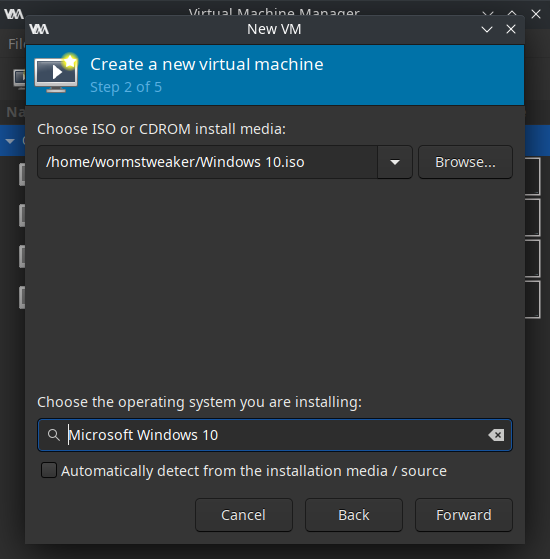
\includegraphics[width=\textwidth]{assets/vmm_iso_selection.png}
\end{minipage}
\begin{minipage}[t]{\linewidth}%
\vspace{0pt}
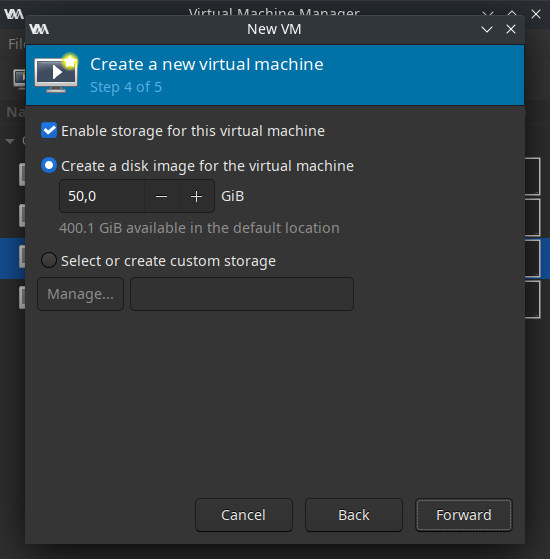
\includegraphics[width=\textwidth]{assets/vmm_disk_creation.png}
\end{minipage}
\end{multicols}

Vamos a asignarle la memoria RAM \emph{(mi recomendación es asignar, como mínimo, 8GB)} a nuestra máquina virtual. Y en el último paso, vamos a elegir el \emph{customizar nuestra máquina virtual antes de la instalación}.

\begin{multicols}{2}
\begin{minipage}[t]{\linewidth}%
\vspace{0pt}
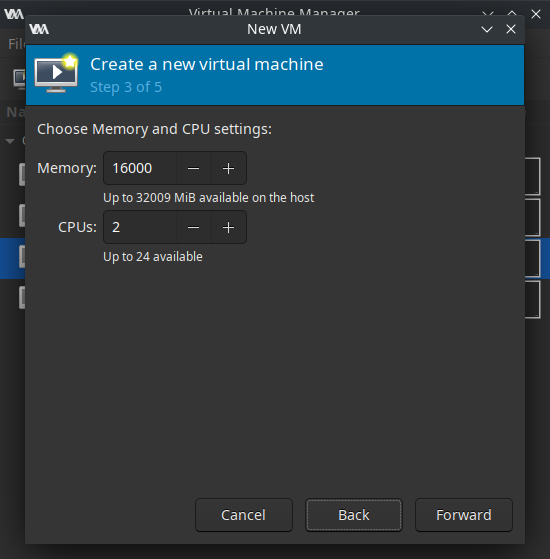
\includegraphics[width=\textwidth]{assets/vmm_memory_setup.png}
\end{minipage}
\begin{minipage}[t]{\linewidth}%
\vspace{0pt}
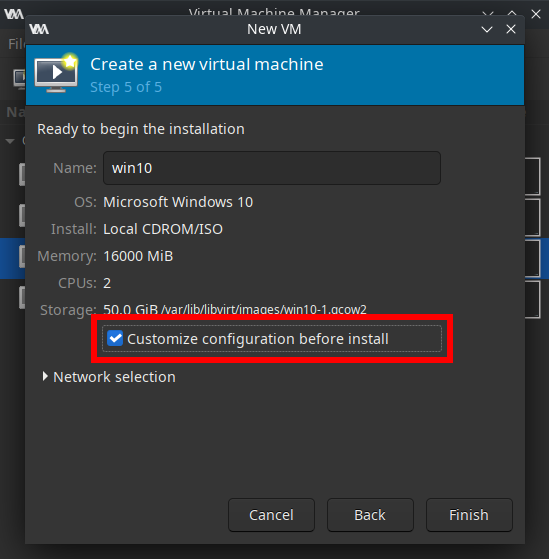
\includegraphics[width=\textwidth]{assets/vmm_name.png}
\end{minipage}
\end{multicols}

Ahora deberás hacer las siguientes modificaciones:

\begin{itemize}
\setlength\itemsep{-0.3em}
\item Cambiar el chipset a \emph{Q35}, y elegir el firmware \emph{UEFI: x86\_64: /usr/share/edk2/x64/OVMF\_CODE.fd}
\item En la pestaña \emph{CPUs} activa el recuadro \emph{Copiar configuración de la CPU del anfitrión}, despliega el menú \emph{Topología} y ajusta la topología de la forma siguiente:
\subitem 1 \emph{Socket}, Tantos \emph{Centros} comos núcleos tenga tu procesador y tantos \emph{Hilos} como hilos tenga tu procesador por núcleo. Por ejemplo para un \emph{i7-10700k} con 8 núcleos y 16 hilos, eligiriamos: \emph{1 Socket, 8 Núcleos, 2 Hilos}. Esto es, si queremos asignar todos los núcleos a nuestra máquina virtual.
\item Nos dirigimos a \emph{SATA Disk 1} y cambiamos el bus a VirtIO, de forma que ahora aparezca \emph{VirtIO Disk 1}. Abrimos las opciones avanzadas, y cambiamos el modo de caché a \emph{writeback}.
\item En los ajustes del \emph{NIC} cambiamos el modelo de dispositivo a \emph{virtio}
\item Por último dale a \emph{Añadir hardware} y añade un almacenamiento de tipo de dispositivo CDROM y escribe al lado de \emph{Administrar...} la localización de el ISO con los drivers virtio, por ejemplo: \emph{/home/usuario/Downloads/virtio-win.iso}.
\end{itemize}

\begin{multicols}{2}
\begin{minipage}[t]{\linewidth}%
\vspace{0pt}
\centering
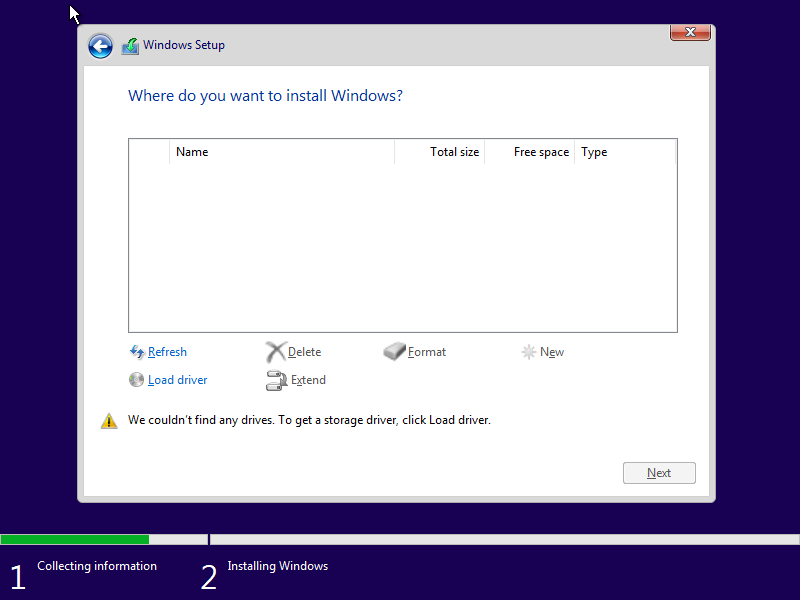
\includegraphics[width=\textwidth]{assets/Screenshot_win10-7.png}
\end{minipage}
\begin{minipage}[t]{\linewidth}%
\vspace{0pt}
\centering
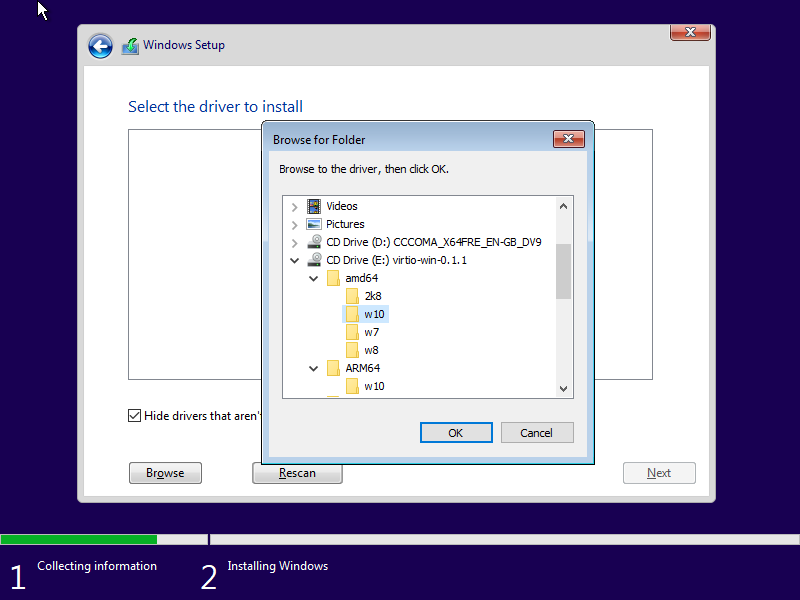
\includegraphics[width=\textwidth]{assets/Screenshot_win10-9.png}
\end{minipage}
\end{multicols}

Dale a \emph{Iniciar la instalación} y cuando veas la selección de disco del instalador de windows verás que está vacío. Primero debes darle a \emph{Cargar driver} o \emph{Load driver}, en inglés.

Selecciona el CD con los drivers virtio y la carpeta que contiene los drivers para Windows 10. Entonces aparecerá tu disco duro virtual y podrás continuar la instalación de Windows. Cuando esta finalize, apaga la máquina virtual.

\begin{multicols}{2}
\begin{minipage}[t]{\linewidth}%
\vspace{0pt}
\centering
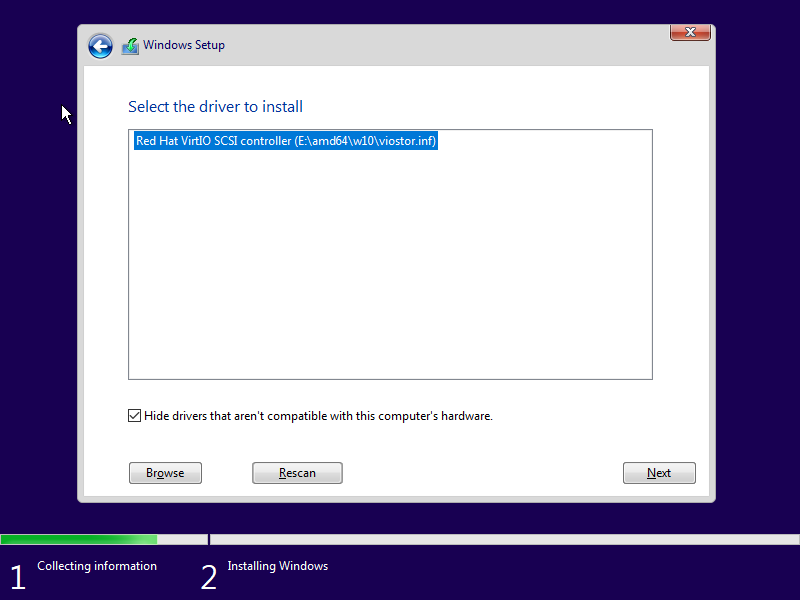
\includegraphics[width=\textwidth]{assets/Screenshot_win10-91.png}
\end{minipage}
\begin{minipage}[t]{\linewidth}%
\vspace{0pt}
\centering
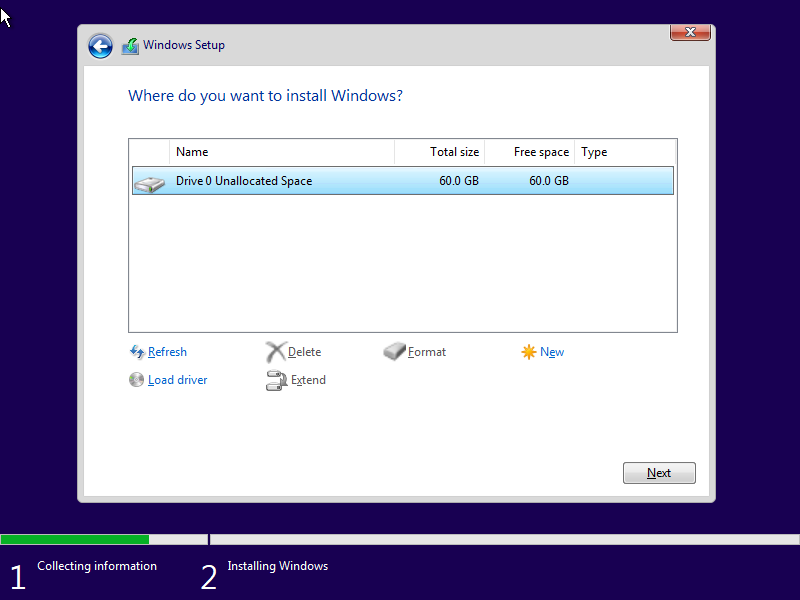
\includegraphics[width=\textwidth]{assets/Screenshot_win10-92.png}
\end{minipage}
\end{multicols}

\subsection{Looking Glass en el Host}

Para poder usar nuestra máquina virtual de forma cómoda vamos a configurar \href{https://looking-glass.io/}{Looking Glass}. Una aplicación que nos permite ver la pantalla conectada a nuestra gráfica através de una ventana y poder controlar nuestra máquina virtual sin necesidad de conectar teclado y ratón a nuestra máquina virtual. El único problema es que para usar looking glass sin necesidad de dos monitores, necesitamos comprar un \href{https://www.amazon.com/s?k=display+dummy}{display dummy}. Por lo menos, su precio suele rondar los 5-7€.

Looking Glass nos muestra una imágen de lo que esta haciendo nuestra gráfica con una latencia muy baja, suficiente para poder jugar a juegos o editar video \emph{(y otros usos posibles)} sin problema en nuestra máquina virtual. Logra esto mandando la información através de un archivo compartido entre máquina virtual y host.

Primero necesitamos configurar \href{dsada}{tmpfilesd} para que cada vez que iniciamos el sistema, cree el archivo que compartiran máquina virtual y host para enviarse información. Tenemos que ejecutar el siguiente comando \emph{(sustituyendo usuario por el nombre de tu usuario)}:

\begin{verbatim}
echo "f /dev/shm/looking-glass 0660 usuario kvm -" | \
doas tee -a /etc/tmpfiles.d/looking-glass.conf
\end{verbatim}

Tenemos que instalar el servicio que se encarga de crear estos archivos con:

\begin{verbatim}
doas pacman -Sy --noconfirm etmpfiles
\end{verbatim}

\subsection{Añadir Gráfica y Looking Glass en el Guest}

Ahora ya tenemos casi todo listo, queda instalar los drivers de video e instalar Looking Glass en nuestra máquina virtual \emph{(a la hora de la instalación debió de haberse instalado ya en nuestro linux)}.

Primero tenemos que añadir nuestra tarjeta gráfica a nuestra máquina virtual. Para ello tenemos que ir a los ajustes de nuestra máquina virtual y en \emph{"Añadir Dispositivo"}

\subsection{Pasos finales}

\begin{mybox}{Nota}
	Para más información sobre como configurar un VFIO passthought puede consultar:
	\begin{itemize}
		\setlength\itemsep{0em}
		\item \href{https://qqq.ninja/blog/post/vfio-on-arch/}{https://qqq.ninja/blog/post/vfio-on-arch/}
		\item \href{https://gitlab.com/risingprismtv/single-gpu-passthrough/-/wikis/home}{https://gitlab.com/risingprismtv/single-gpu-passthrough/-/wikis/home}
		\item \href{https://wiki.archlinux.org/title/PCI\_passthrough\_via\_OVMF}{https://wiki.archlinux.org/title/PCI\_passthrough\_via\_OVMF}
	\end{itemize}
\end{mybox}

\section{GRUB config}

\label{sec:tsc}

Para un mayor rendimiento es recomendable añadir a las opciones de arranque de GRUB \emph{tsc-reliable} y \emph{clocksource=tsc}:

\begin{verbatim}
GRUB_CMDLINE_LINUX="tsc-reliable clocksource=tsc"
\end{verbatim}

También esto ayuda a que el script \ref{sec:wake} funcione correctamente.

\section{SSH}

Si queremos conectarnos a un equipo remoto atraves de internet debemos configurar \href{https://es.wikipedia.org/wiki/OpenSSH}{OpenSSH}, podemos activar el servicio con:

\begin{verbatim}
doas rc-update add sshd default
\end{verbatim}

Pero antes vamos a seguir una serie de pasos, pues la configuración por defecto no es muy segura.

...

\subsection{VNC através de SSH}

Podemos usar SSH para acceder a nuestro entorno gráfico de forma remota y usar nuestro ordenador sin estar necesariamente delante de el físicamente. Por defecto dwm inicia un servidor \href{https://en.wikipedia.org/wiki/Virtual_Network_Computing}{VNC} para que puedas conectarte remotamente a una interfaz gráfica. Para poder hacer uso del servidor VNC tienes que usar \href{https://en.wikipedia.org/wiki/Tunneling_protocol}{tunneling}. Para conectarte y poder usar VNC, ejecuta:

\begin{verbatim}
ssh usuario1@255.255.255.255 -L 5900:localhost:5900
\end{verbatim}

Sustituye \emph{usuario1} por el usuario de tu máquina, y \emph{255.255.255.255} por la dirección IP de tu máquina.

Para conectarte a tu torre debes tener instalado algun cliente VNC, mi recomendación es \href{https://github.com/FreeRDP/Remmina}{remmina}. Abre tu cliente VNC y conectate a \emph{localhost:5900}, eso es todo.

\section{Firewall}

Instalar y configurar un firewall no es posible dentro de un chroot. Por eso configurar el firewall debe hacerse una vez reiniciemos y hallamos arrancado nuestro sistema operativo. Para instalar el firewall ejecuta:

\begin{verbatim}
doas sh -c 'pacman -Sy ufw-openrc; rc-update add ufw default; ufw enable'
\end{verbatim}

Ahora, la próxima vez que inicies tu equipo tendras un firewall ya instalado. Para configurarlo puedes ejecutar los siguientes comandos, que establecen unas reglas de filtrado de paquetes bastante permisivas.

\begin{verbatim}
doas ufw limit 22/tcp
doas ufw allow 80/tcp
doas ufw allow 443/tcp
doas ufw allow syncthing
doas ufw default deny incoming
doas ufw default allow outgoing
\end{verbatim}

\section{Syncthing}

\href{https://github.com/syncthing/syncthing}{Syncthing} es un software para sincronizar archivos entre dispositivos, es lo que uso para poder trabajar en todos mis equipos sin necesidad de estar intercambiando pen-drives como un troglodita.

Viene instalado por defecto y se ejecuta cuando inicias tu ordenador. Para configurarlo tiene una \href{http://localhost:8384/}{interfaz gráfica} a la que puedes acceder desde tu navegador.

\begin{mybox}{Información}
Aquí puedes encontrar documentación sobre como usar syncthing: \href{https://docs.syncthing.net/}{https://docs.syncthing.net/}
\end{mybox}


\section{Monitores de altas tasas de refresco}

Por defecto dwm actualiza el movimiento de las ventanas a 60fps. Si tienes un monitor de mas de 60Hz esto puede hacer la experiencia de usar dwm insatisfactoria. Para cambiar este comportamiento, debes editar el archivo \emph{dwm.c}, primero debes ir a la función:

\begin{verbatim}
void
movemouse(const Arg *arg)
\end{verbatim}

Encontrar las lineas:

\begin{verbatim}
    break;
case MotionNotify:
    if ((ev.xmotion.time - lasttime) <= (1000 / 60))
        continue;
    lasttime = ev.xmotion.time;
\end{verbatim}

Y cambiar el valor 60 por la tasa de refresco de tu monitor. Por ejemplo, para un monitor de 144Hz, la línea a cambiar debería verse así:

\begin{verbatim}
if ((ev.xmotion.time - lasttime) <= (1000 / 144))
\end{verbatim}

Ahora debes encontrar la misma línea en:

\begin{verbatim}
void
resizemouse(const Arg *arg)
\end{verbatim}

y realizar el mismo tipo de modificación. Para hacer los cambios efectivos re-compila dwm ejecutando \emph{doas make install} desde la carpeta de dwm, y reinicia dwm pulsando \emph{Alt Izq. + Shift + F11}.

\end{document}
